\subsection*{Problema 4b}

\textbf{Interpola la curva paramétria de la ecuación \ref{eq:ft_problma4b}.}

\begin{equation}
	f(t) = (r(t)sin(t),r(t)cos(t)) \label{eq:ft_problma4b}
\end{equation}

\textbf{donde}

\begin{equation*}
	r(t) = exp(cos(t)-2cos(4t)+sin\left (\frac{t}{12}\right )^5
\end{equation*}

\textbf{a partir de 25 puntos definidos en la ecuación \ref{eq:points_4b}.}

\begin{equation}
	(x_i,y_i) = (x(t_i),y(t_i)) \qquad t_i = \frac{\pi i}{12} \qquad i=0,1,2,\dots,24 \label{eq:points_4b}
\end{equation}


Se modifico la ecuación \ref{eq:points_4b} de la siguiente manera:

\begin{equation}
	(x_i,y_i) = (x(t_i),y(t_i)) \qquad t_i = \frac{25\pi i}{12n} \qquad i=0,1,2,\dots,n \label{eq:points_4b_modificado}
\end{equation}

Esto para tener diferentes cantidades de puntos entre el valor mínimo y máximo de la ecuación \ref{eq:points_4b}.

En la gráfica \ref{fig:problem4b} se encuentran los resultados de  la interpolación usando $n=\{10,25,50,100\}$
\begin{figure}[H]
	\centering
	\begin{subfigure}[b]{8cm}
		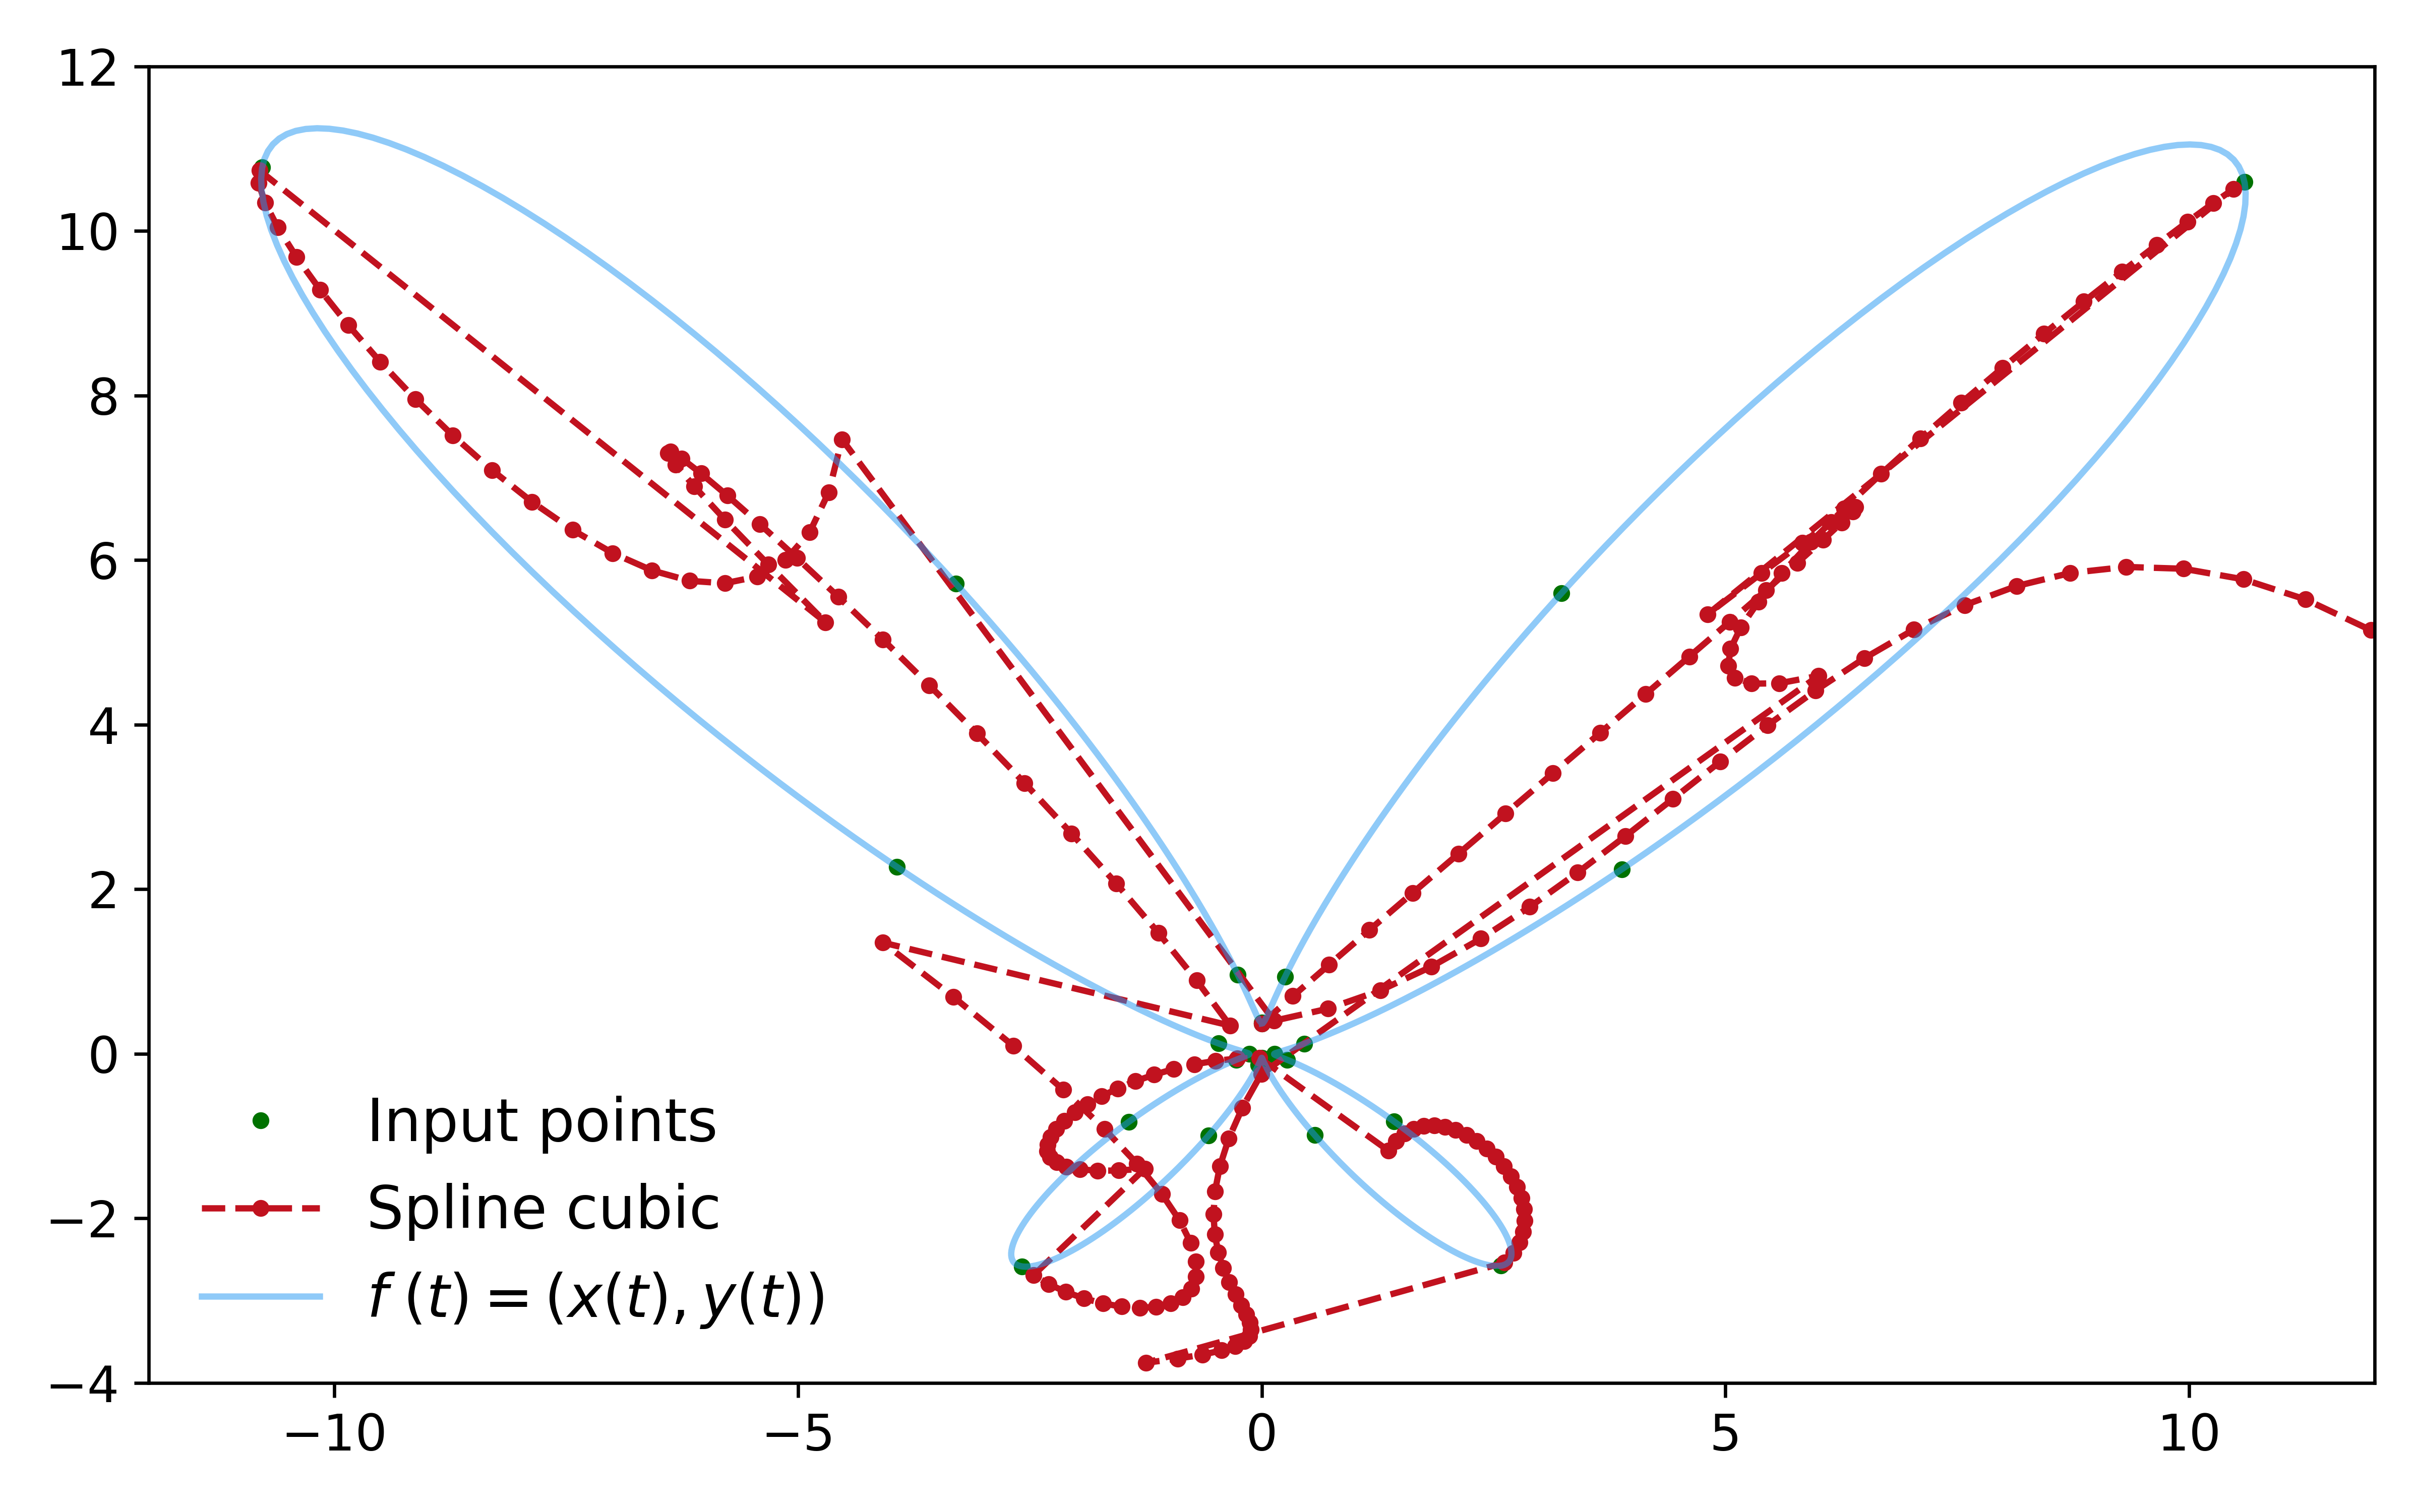
\includegraphics[width=8cm]{Graphics/problema04b_10.png}
		\caption{$n=10$.}
		\label{fig:problem4b10}
	\end{subfigure}
	\begin{subfigure}[b]{8cm}
		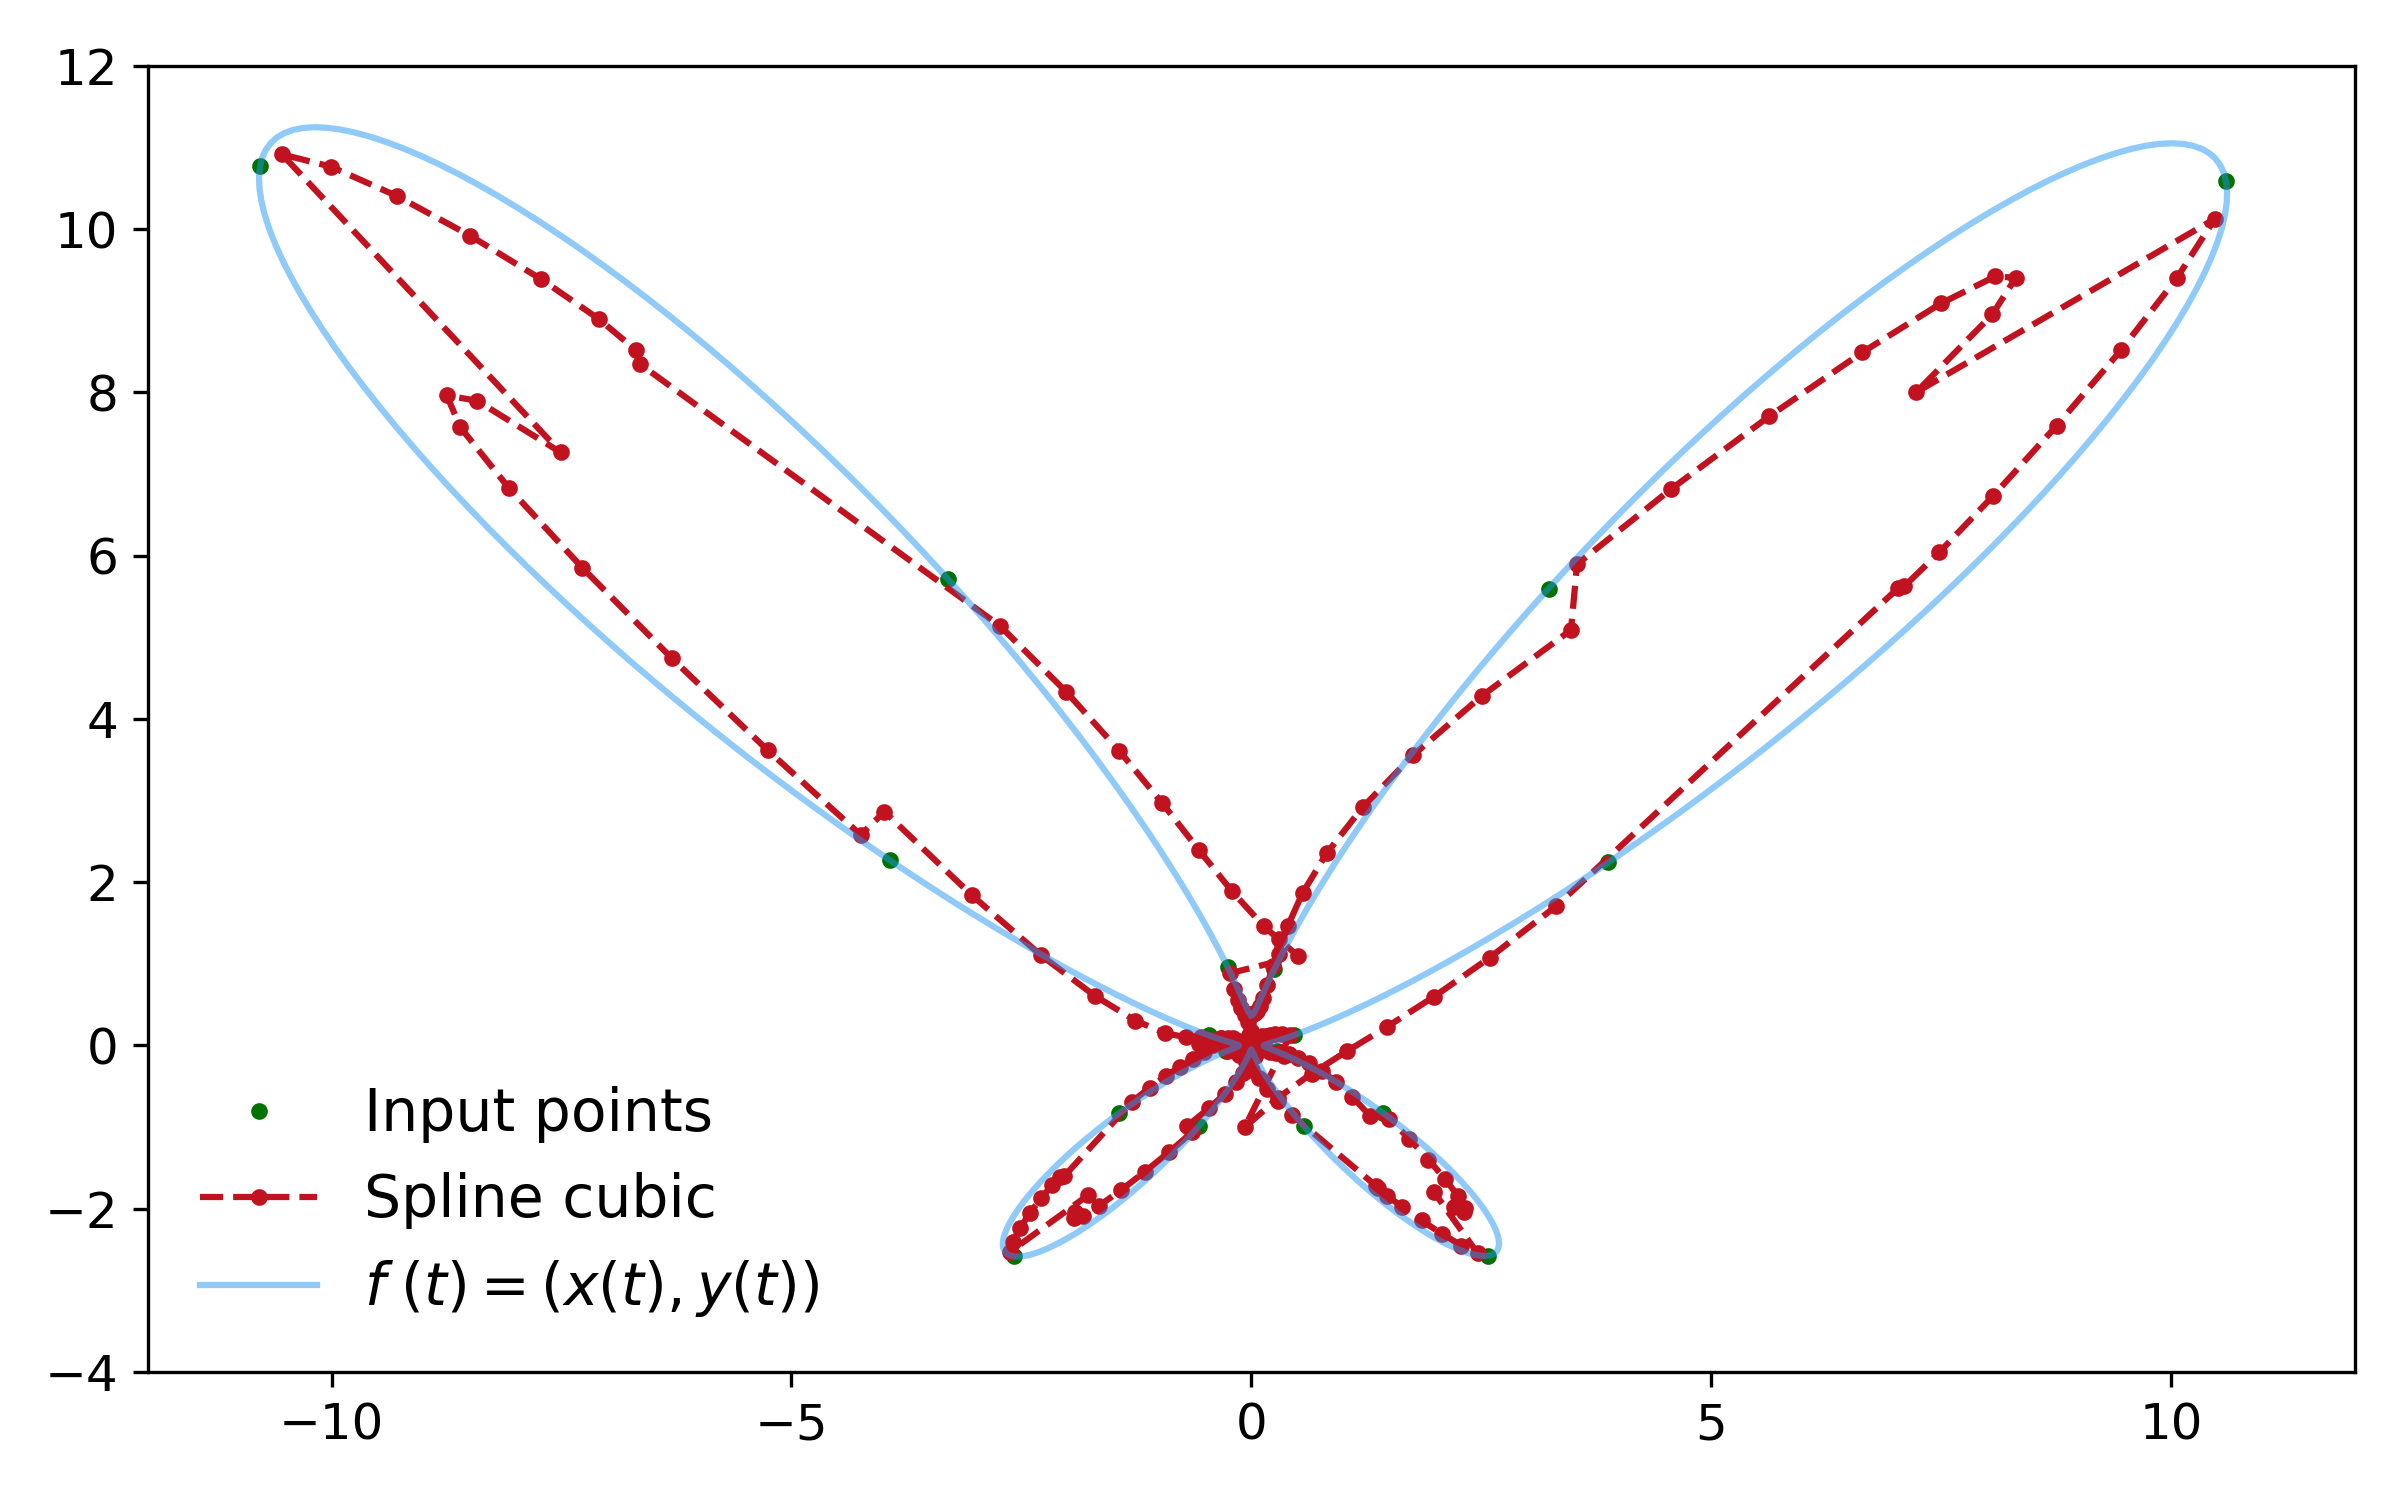
\includegraphics[width=8cm]{Graphics/problema04b_25.png}
		\caption{$n=25$.}
		\label{fig:problem4b25}
	\end{subfigure}
	\begin{subfigure}[b]{8cm}
		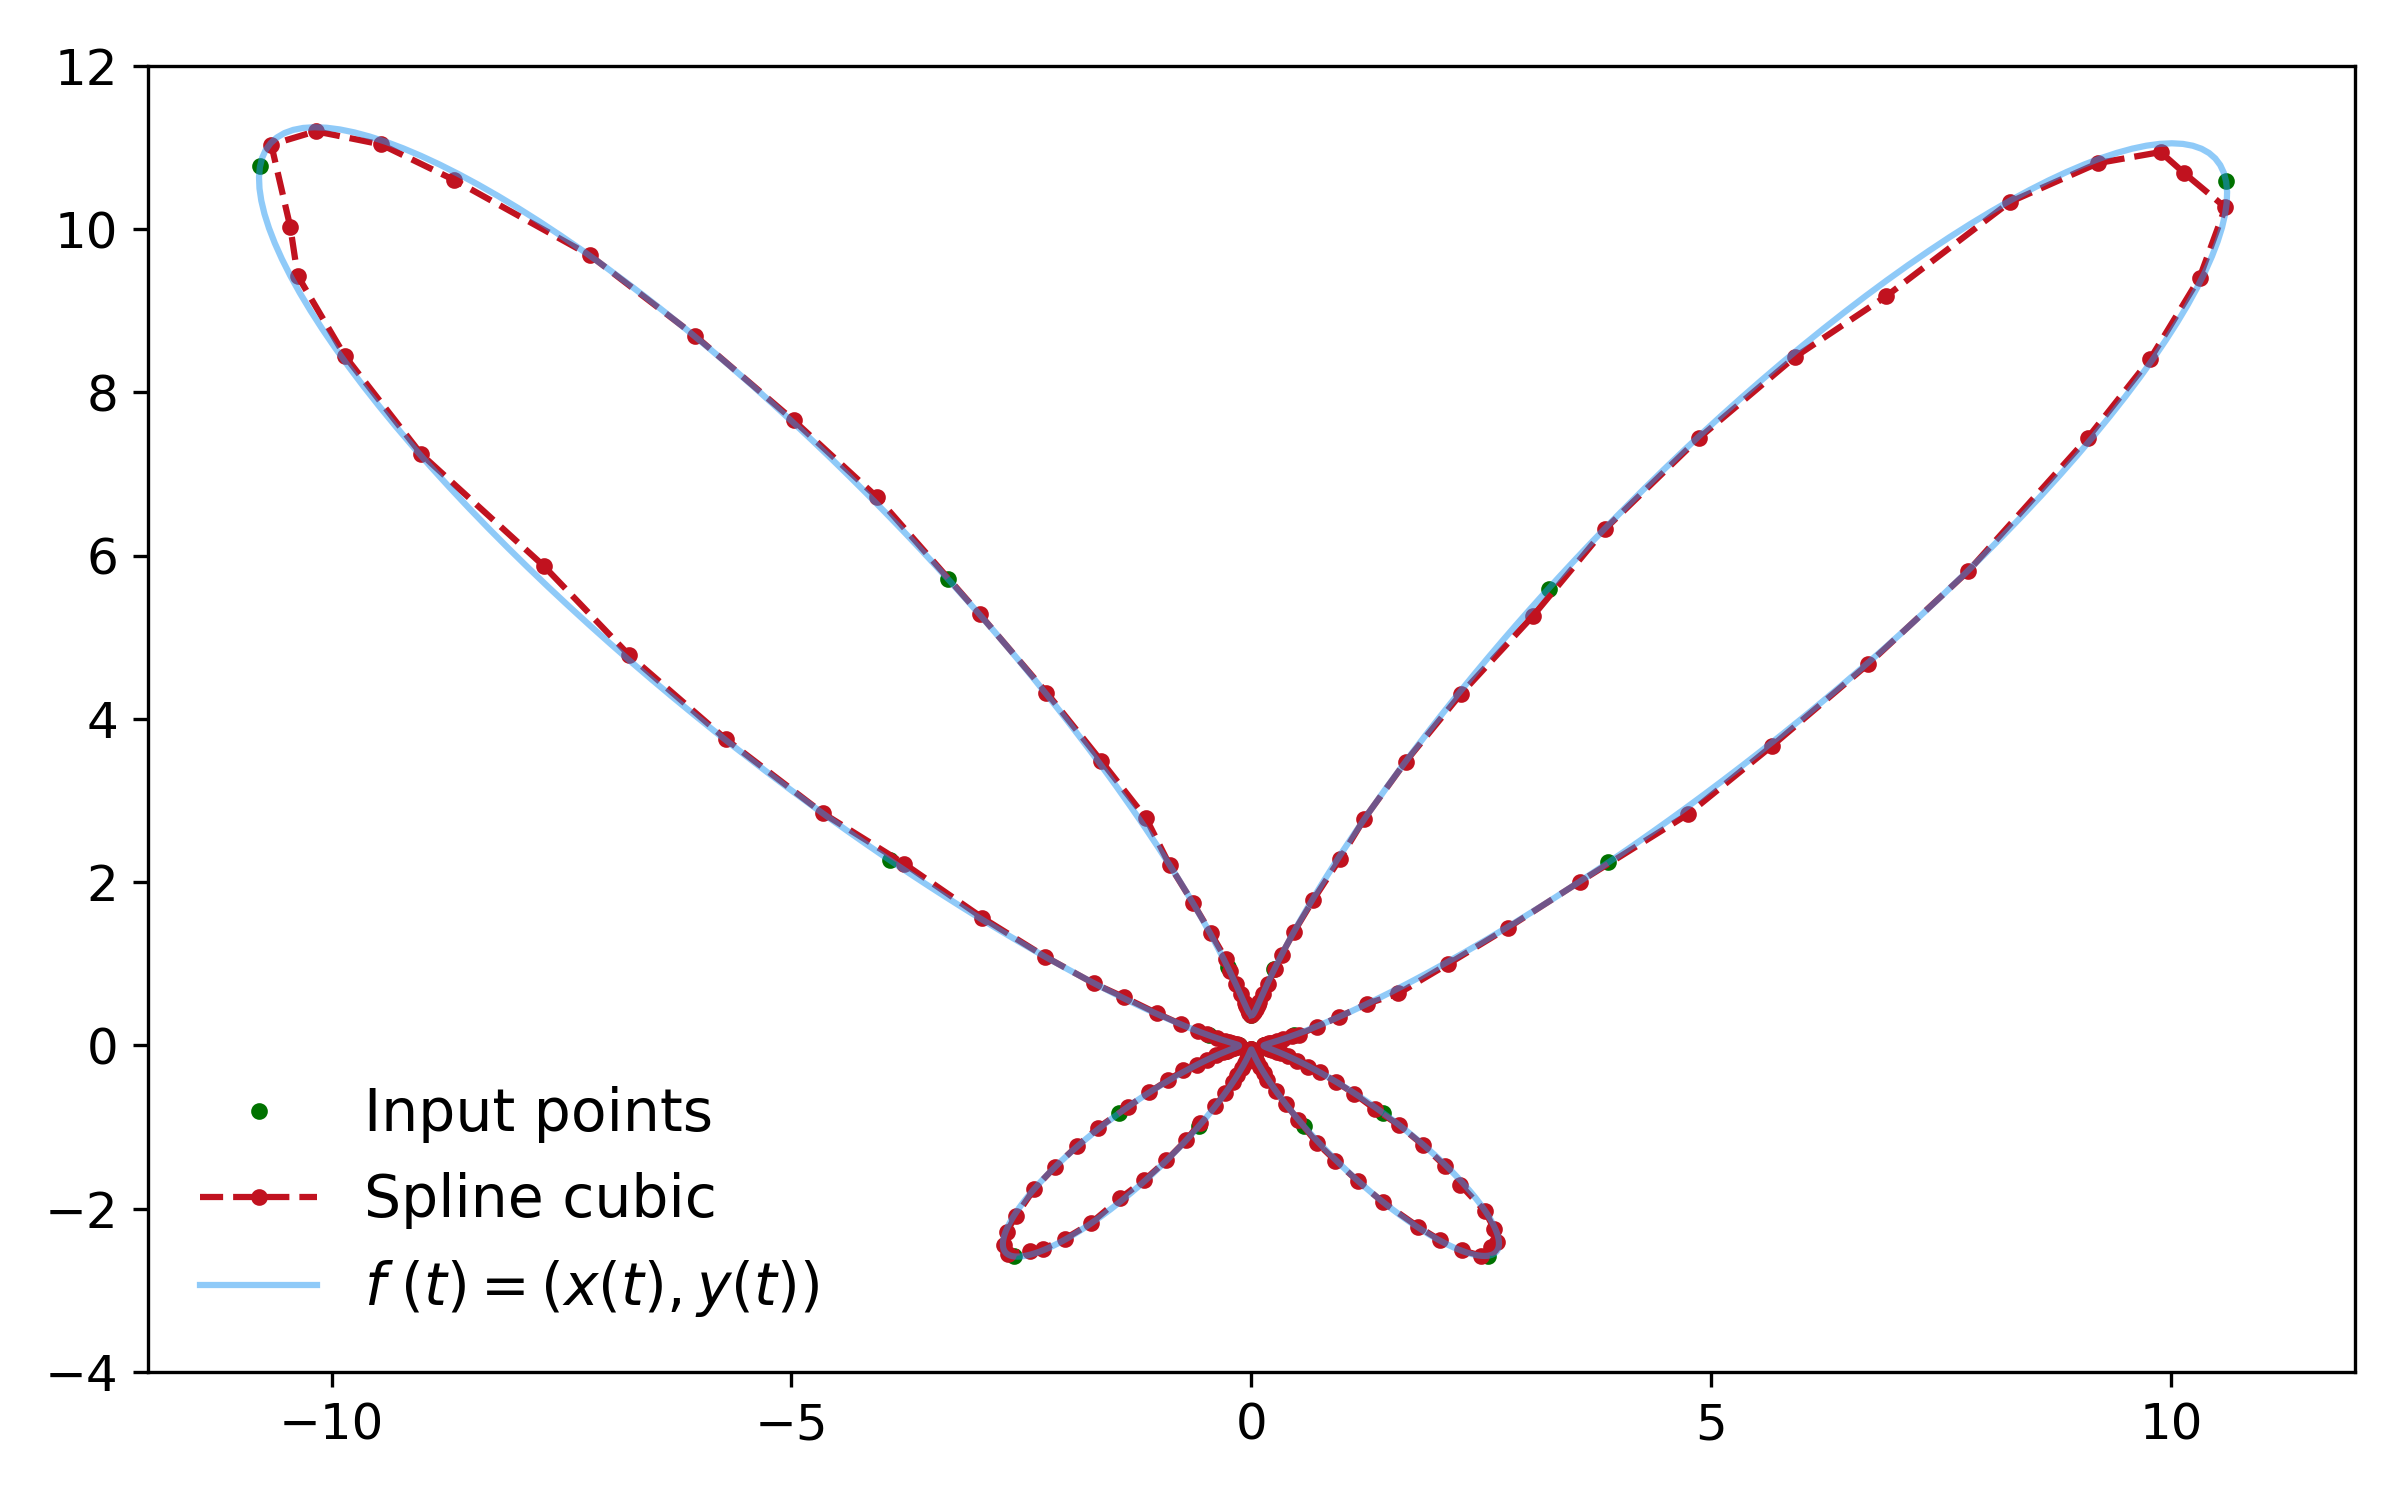
\includegraphics[width=8cm]{Graphics/problema04b_50.png}
		\caption{$n=50$.}
		\label{fig:problem4b50}
	\end{subfigure}
	\begin{subfigure}[b]{8cm}
		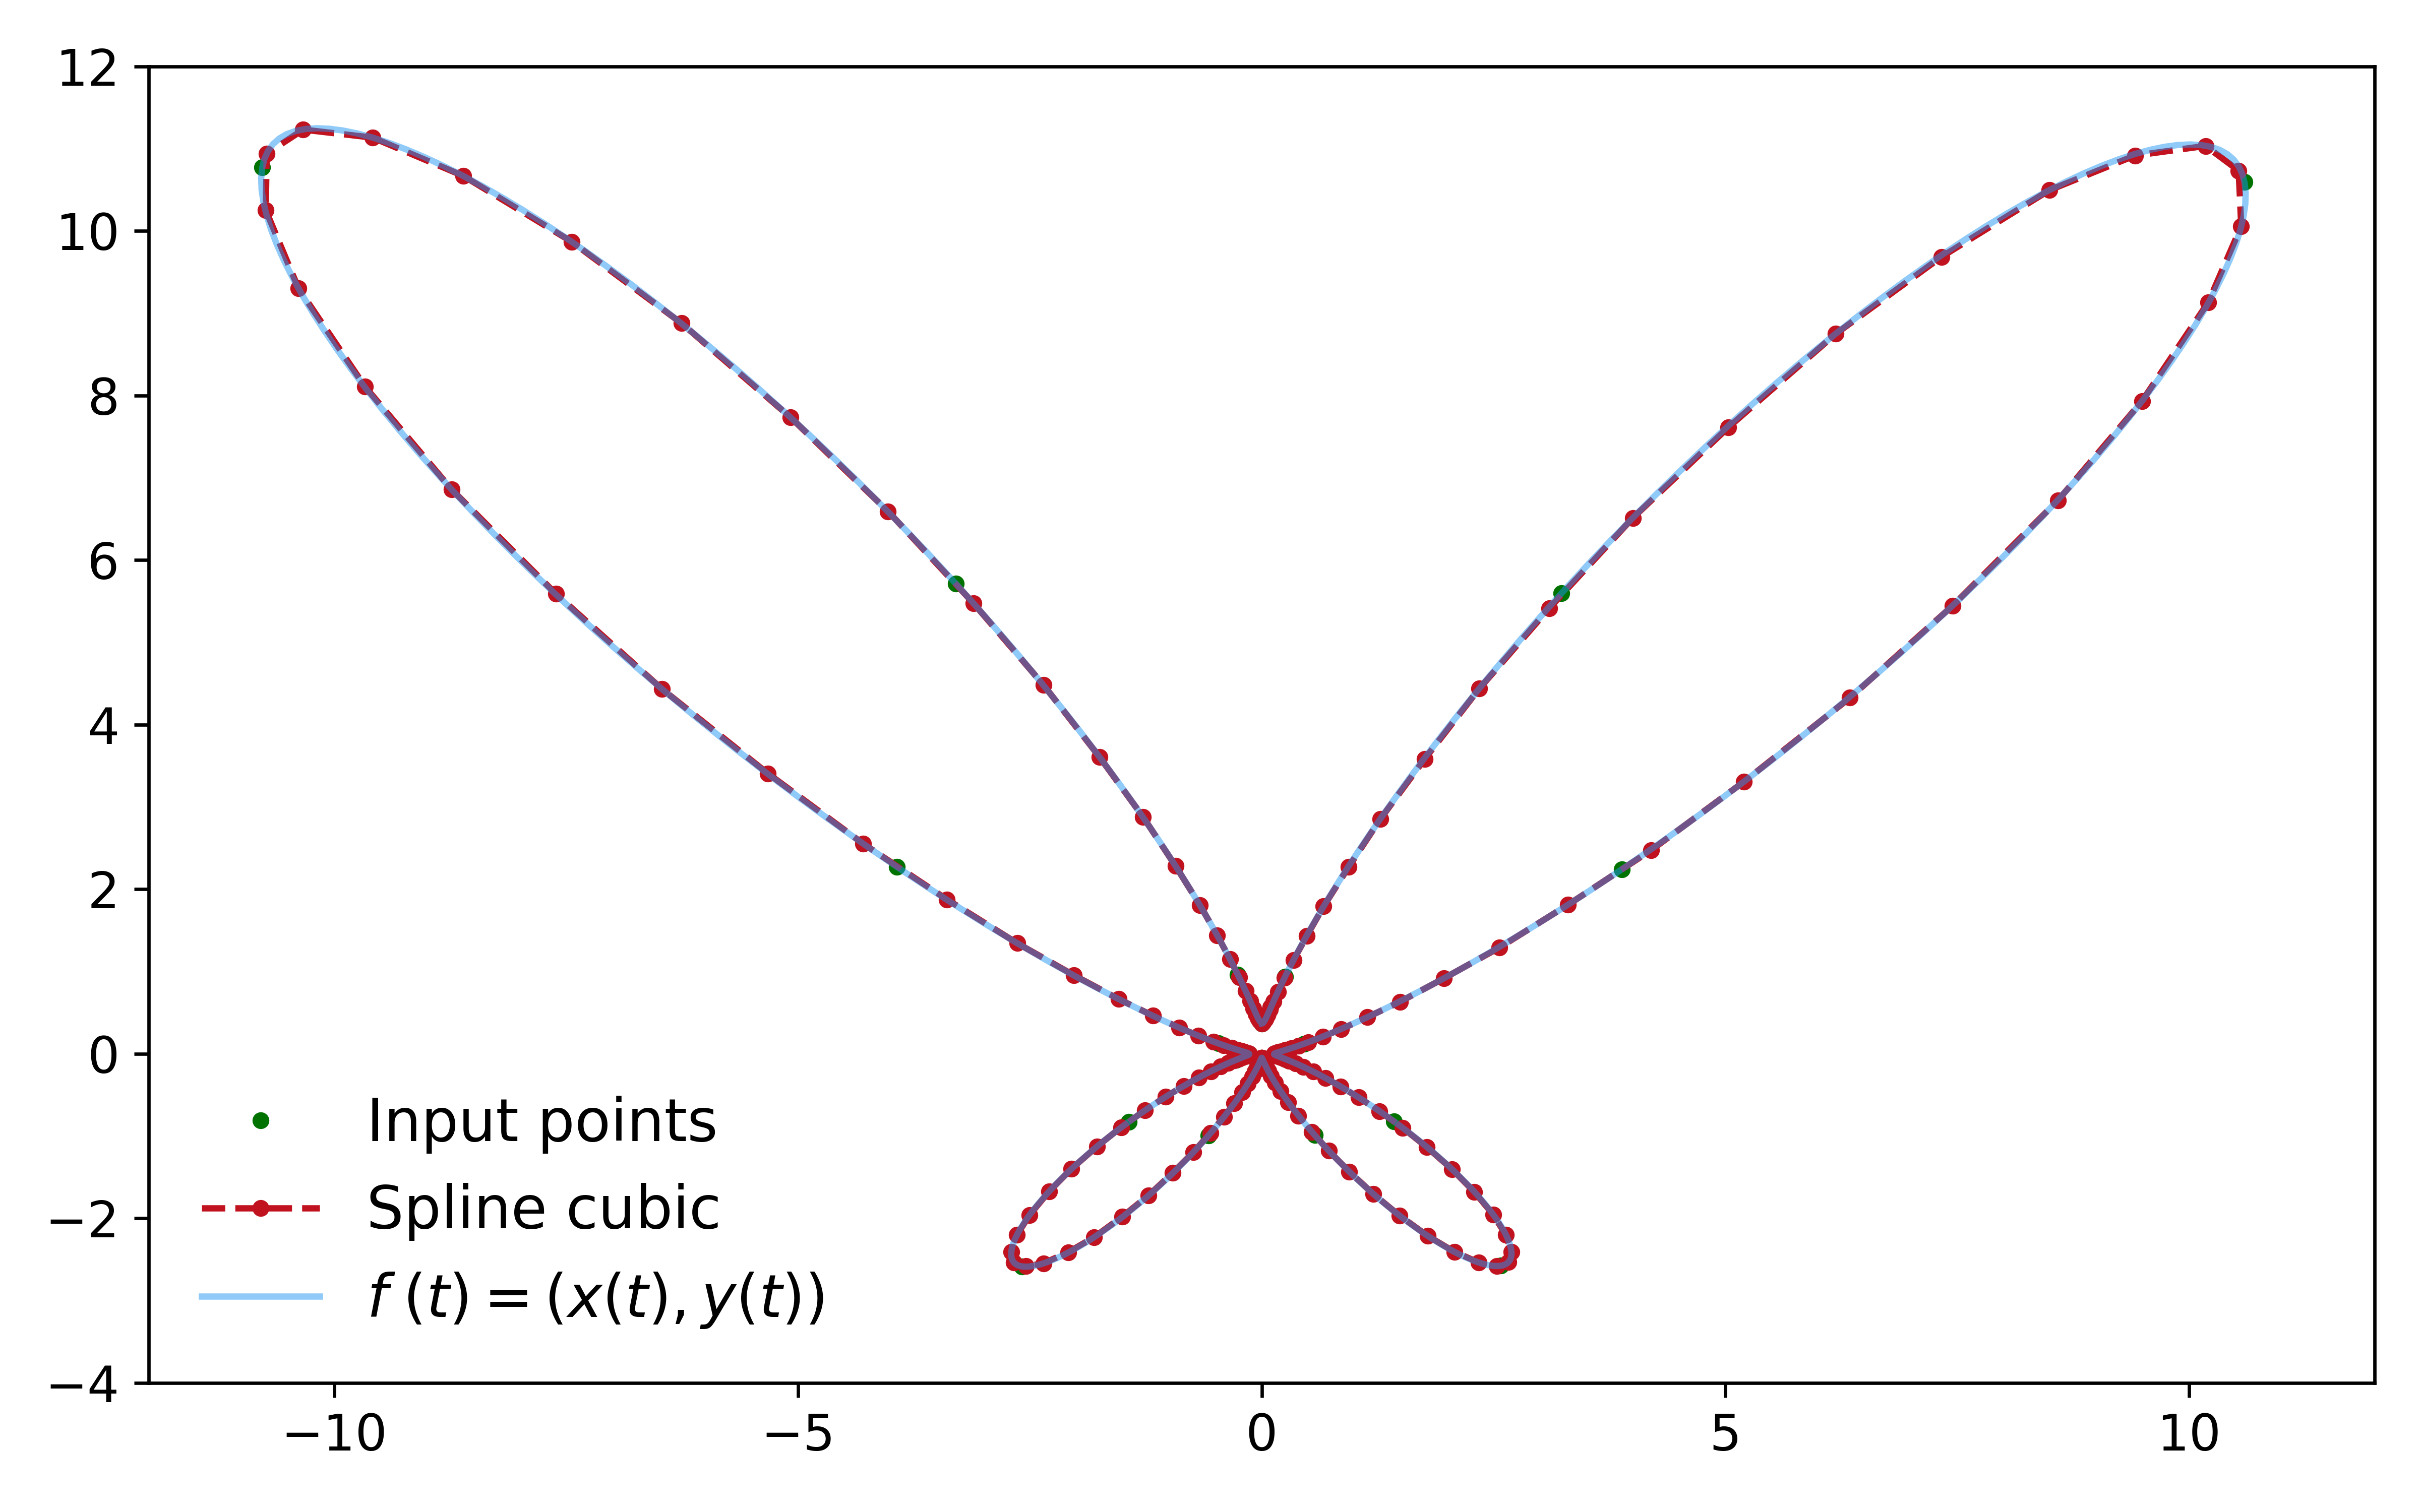
\includegraphics[width=8cm]{Graphics/problema04b_100.png}
		\caption{$n=100$.}
		\label{fig:problem4b100}
	\end{subfigure}
	\caption{Ecuación \ref{eq:ft_problma4b} y  \ref{eq:points_4b_modificado} con para diferentes cantidades de puntos como input.}
	\label{fig:problem4b}
\end{figure}

En las gráficas \ref{fig:problem4b10} y \ref{fig:problem4b25} se aprecia que la falta de información en central y superior provoca que la interpolación sea diferente a la ecuación real, siendo la gráfica \ref{fig:problem4b10} la que contiene una mayor diferencia. Con esto se llega a la conclusión que mientras más sean los puntos que se conocen de la función la interpolación se acercará a la función original.

Realizando un acercamiento a la zona $[-2,2]\times[-2,2]$ se obtiene la gráfica \ref{fig:problema4b_zoom}.

\begin{figure}[H]
	\centering
	\begin{subfigure}[b]{8cm}
		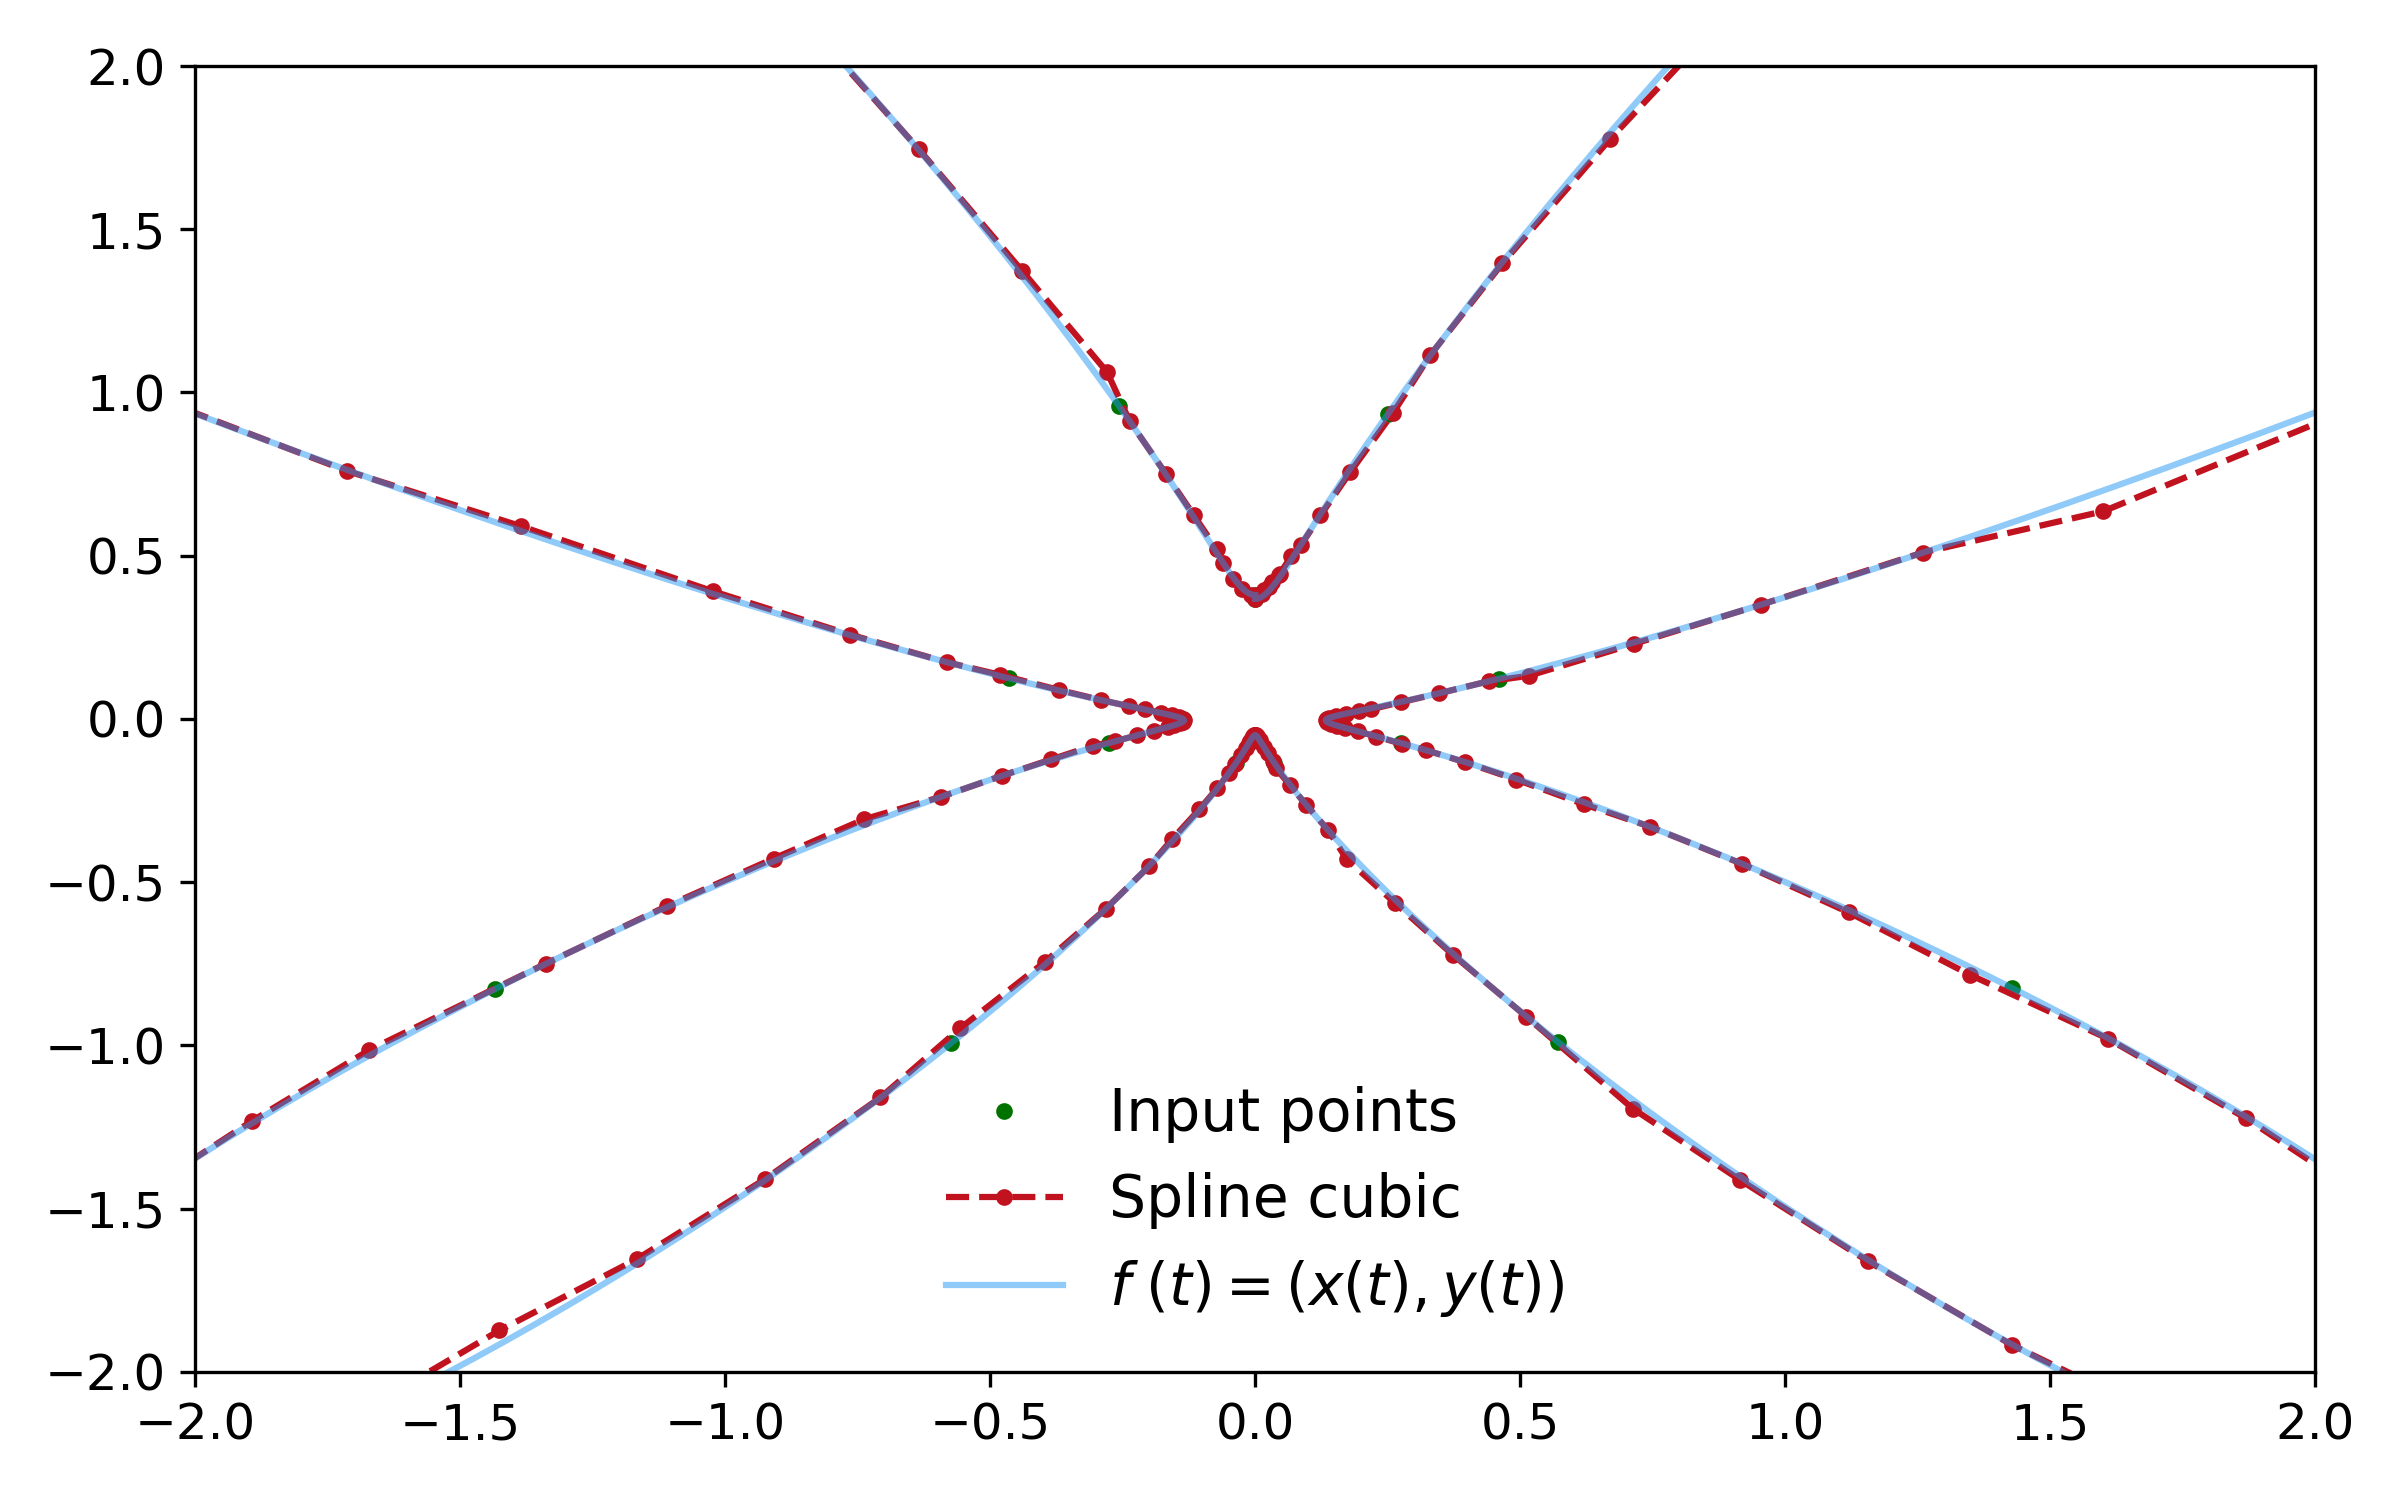
\includegraphics[width=8cm]{Graphics/problema04b_zoom50.png}
		\caption{$n=50$.}
		\label{fig:problema4b_zoom50}
	\end{subfigure}
	\begin{subfigure}[b]{8cm}
		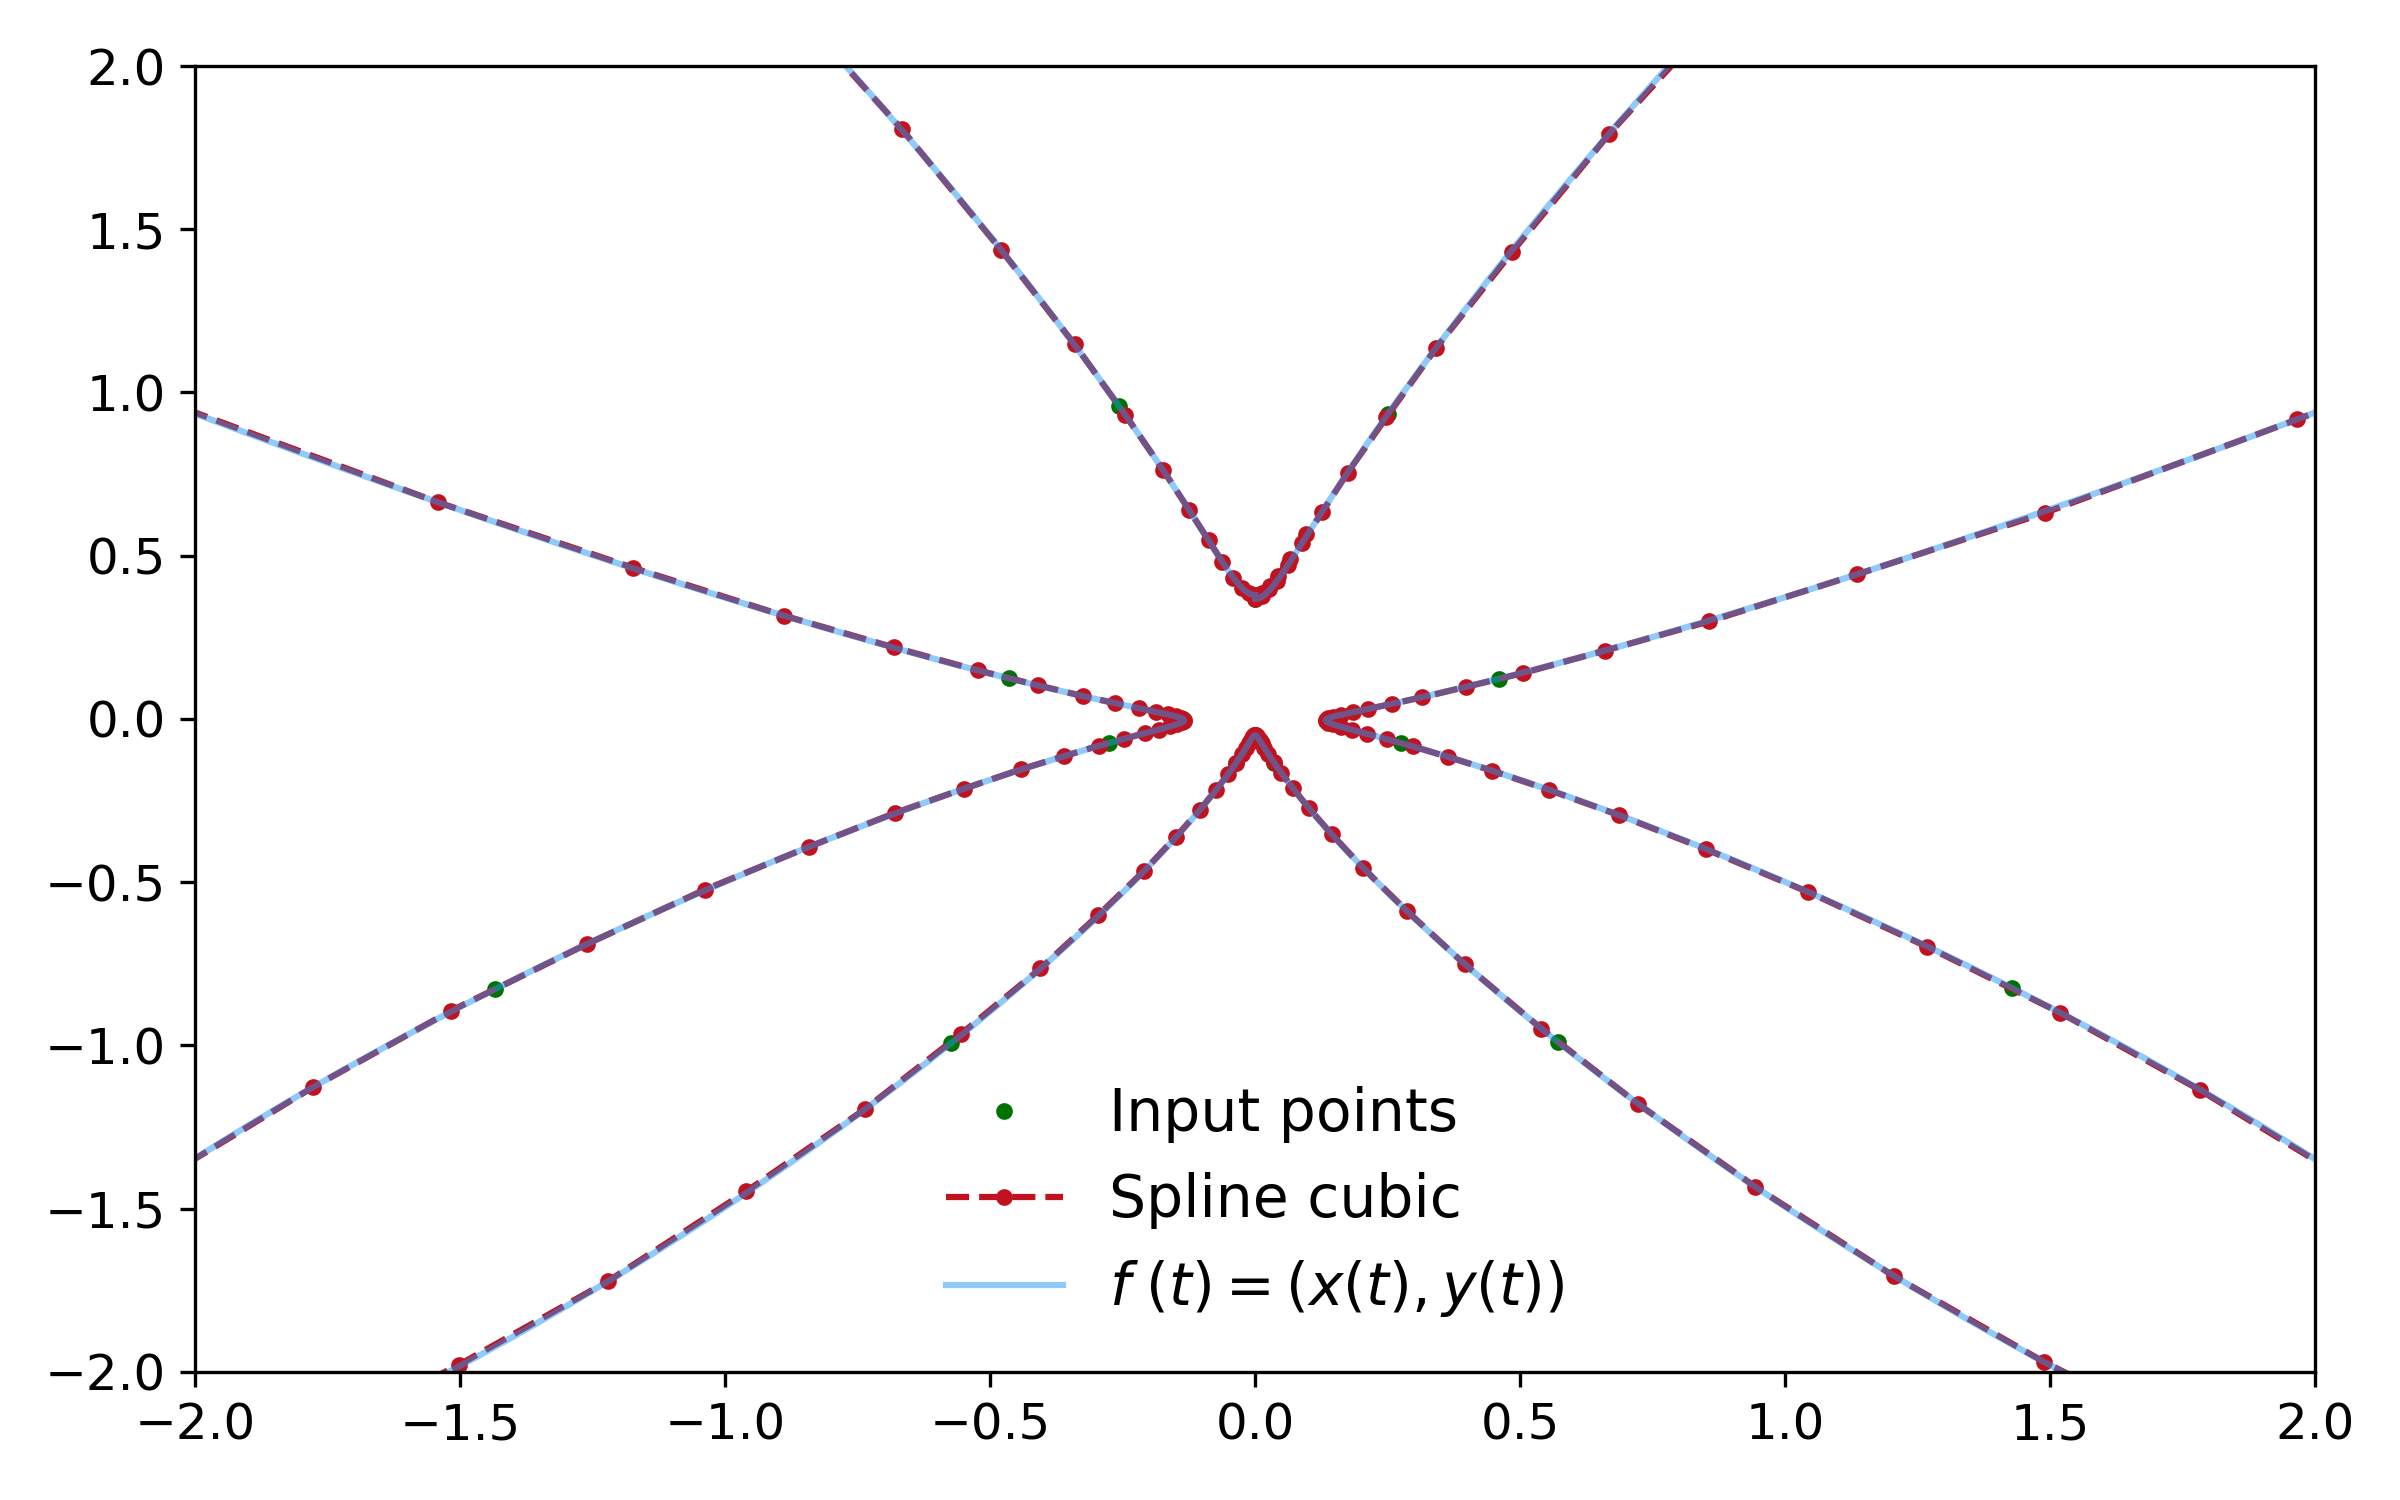
\includegraphics[width=8cm]{Graphics/problema04b_zoom100.png}
		\caption{$n=100$}
		\label{fig:problema4b_zoom100}
	\end{subfigure}
	\caption{Ecuación \ref{eq:ft_problma4b} en la zona $[-2,2]\times[-2,2]$.}
	\label{fig:problema4b_zoom}
\end{figure}

En la gráfica \ref{fig:problema4b_zoom} se logra visualizar la diferencia a detalle para el uso de $n=\{50,100\}$. La gráfica \ref{fig:problema4b_zoom50} contiene diferencias con respecto a la función original, las cuales la gráfica \ref{fig:problema4b_zoom100} no presenta. Estas diferencias son muy mínimas al punto en que son aceptables, ya que la cantidad de puntos para obtener esa apŕoximación es la mitad de la otra.
\pagebreak
